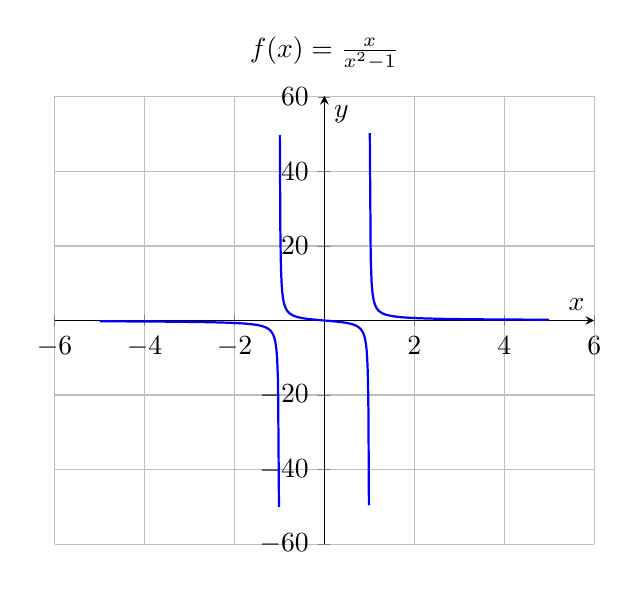
\begin{tikzpicture}
    \begin{axis}[
        title={$f(x) = \frac{x}{x^2 - 1}$},
        axis lines = middle,
        grid = major,
        enlargelimits = true,
        xlabel={$x$},
        ylabel={$y$},
    ]

    % Intervalo 1: desde -5 hasta un poco antes de -1
    \addplot[domain=-5:-1.01, samples=200, thick, blue] {x/(x^2 - 1)};

    % Intervalo 2: de -0.99 hasta 0.99 (separa la zona cerca de ±1)
    \addplot[domain=-0.99:0.99, samples=200, thick, blue] {x/(x^2 - 1)};

    % Intervalo 3: de 1.01 hasta 5
    \addplot[domain=1.01:5, samples=200, thick, blue] {x/(x^2 - 1)};

    \end{axis}
\end{tikzpicture}
